\section{Results}
\label{sec:results}
\paragraph{Performance metrics}


In the case of the narration data this scores is not confounded by
speaker-based clues, which is an indication that the model possibly
learned to detect some aspects of utterance meaning. 

\begin{figure*}[htb]
  \centering
  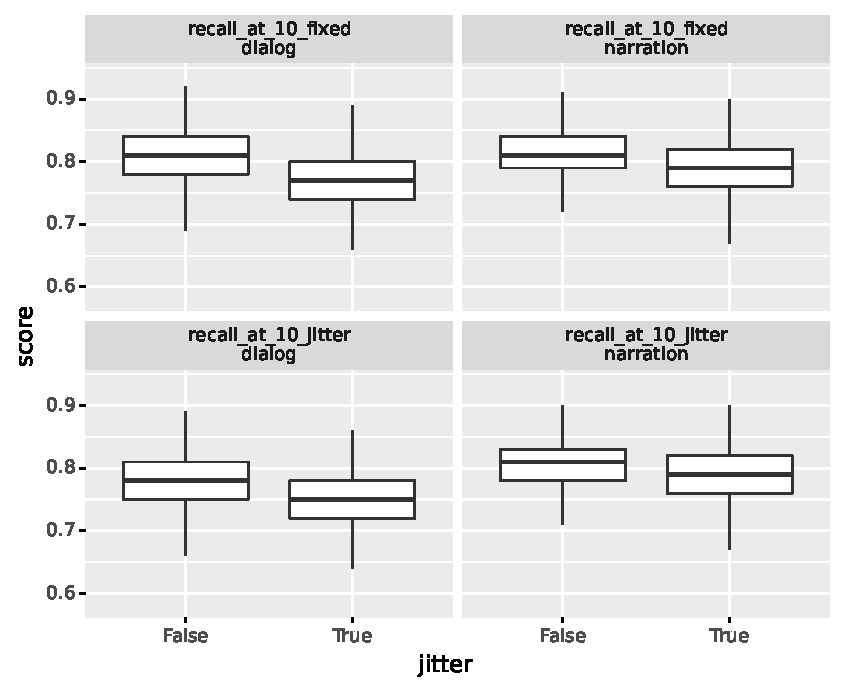
\includegraphics[width=0.9\textwidth]{results/ablations/jitter.pdf}
  \caption{Effect of jitter.}
  \label{fig:jitter}
\end{figure*}

\begin{figure*}[htb]
  \centering
  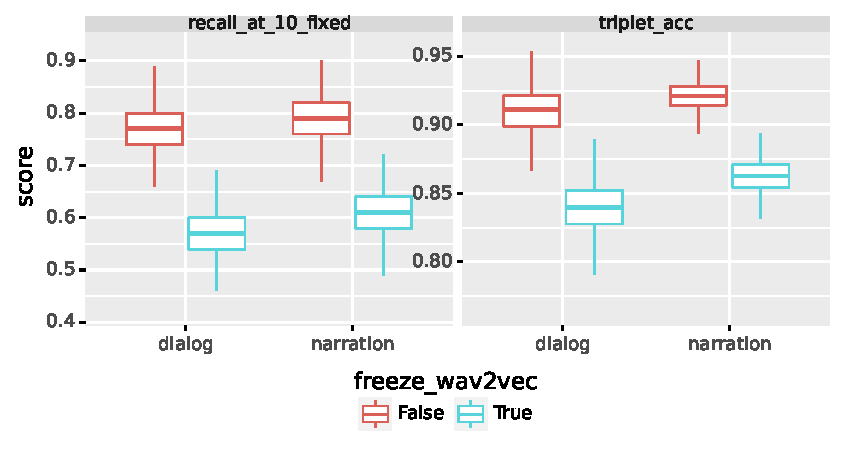
\includegraphics[width=0.9\textwidth]{results/ablations/freeze_wav2vec.pdf}
  \caption{Effect of freezing the parameters of the \textsc{wav2vec} module.}
  \label{fig:freeze_wav2vec}
\end{figure*}

\begin{figure*}[htb]
  \centering
  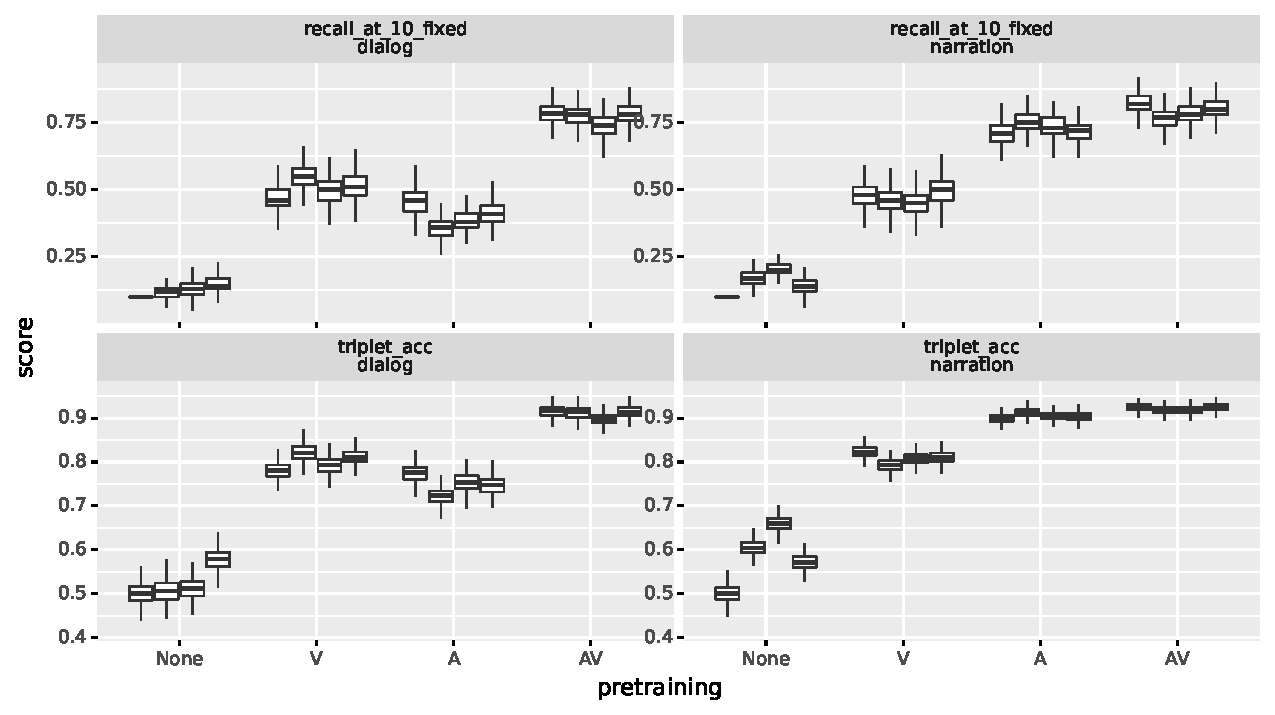
\includegraphics[width=0.9\textwidth]{results/ablations/pretraining.pdf}
  \caption{Effect of pre-training.}
  \label{fig:pretraining}
\end{figure*}

\begin{figure*}[htb]
  \centering
  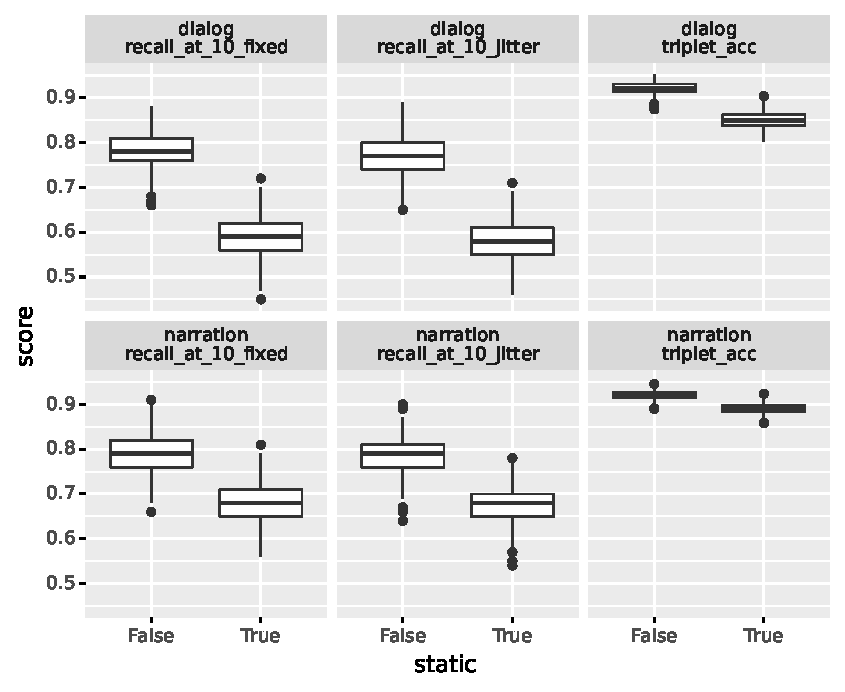
\includegraphics[width=0.9\textwidth]{results/ablations/static.pdf}
  \caption{Effect of temporal information.}
  \label{fig:static}
\end{figure*}


\paragraph{Targeted Triplets}
As a first baseline, we evaluate a model that has been pretrained but not fine-tuned on our dataset. The resulting performance is, as expected, close to chance level: 0.538.\todo{MN: add baselines: model that is completely untrained, and model where only the attention pooling layers are finetuned} Additionally, we evaluate a model that is trained using static (image) data instead of video. The average accuracy is 0.705 . Finally, the best performing model according to the
performance metrics (ID 68, audio and video pretraining) achieves an average
targeted triplets accuracy of 0.745.

\Cref{fig:accuracy_targeted_triplets_nouns} and
\ref{fig:accuracy_targeted_triplets_verbs} show per-word
accuracy for nouns and verbs, respectively. We perform boostrapping (n\_resampling = 100) to estimate mean and standard deviation for each accuracy score.

We further compute correlations between the per-word accuracy and two possible predictors of age of acquisition: frequency and concreteness. The resulting correlations are presented in Appendix \ref{app:targeted_triplets_eval}. We do not find any significant correlation between the model's per-word accuracy and word concreteness or input frequency of a word in the training data.




\begin{figure*}[htb]
  \centering
  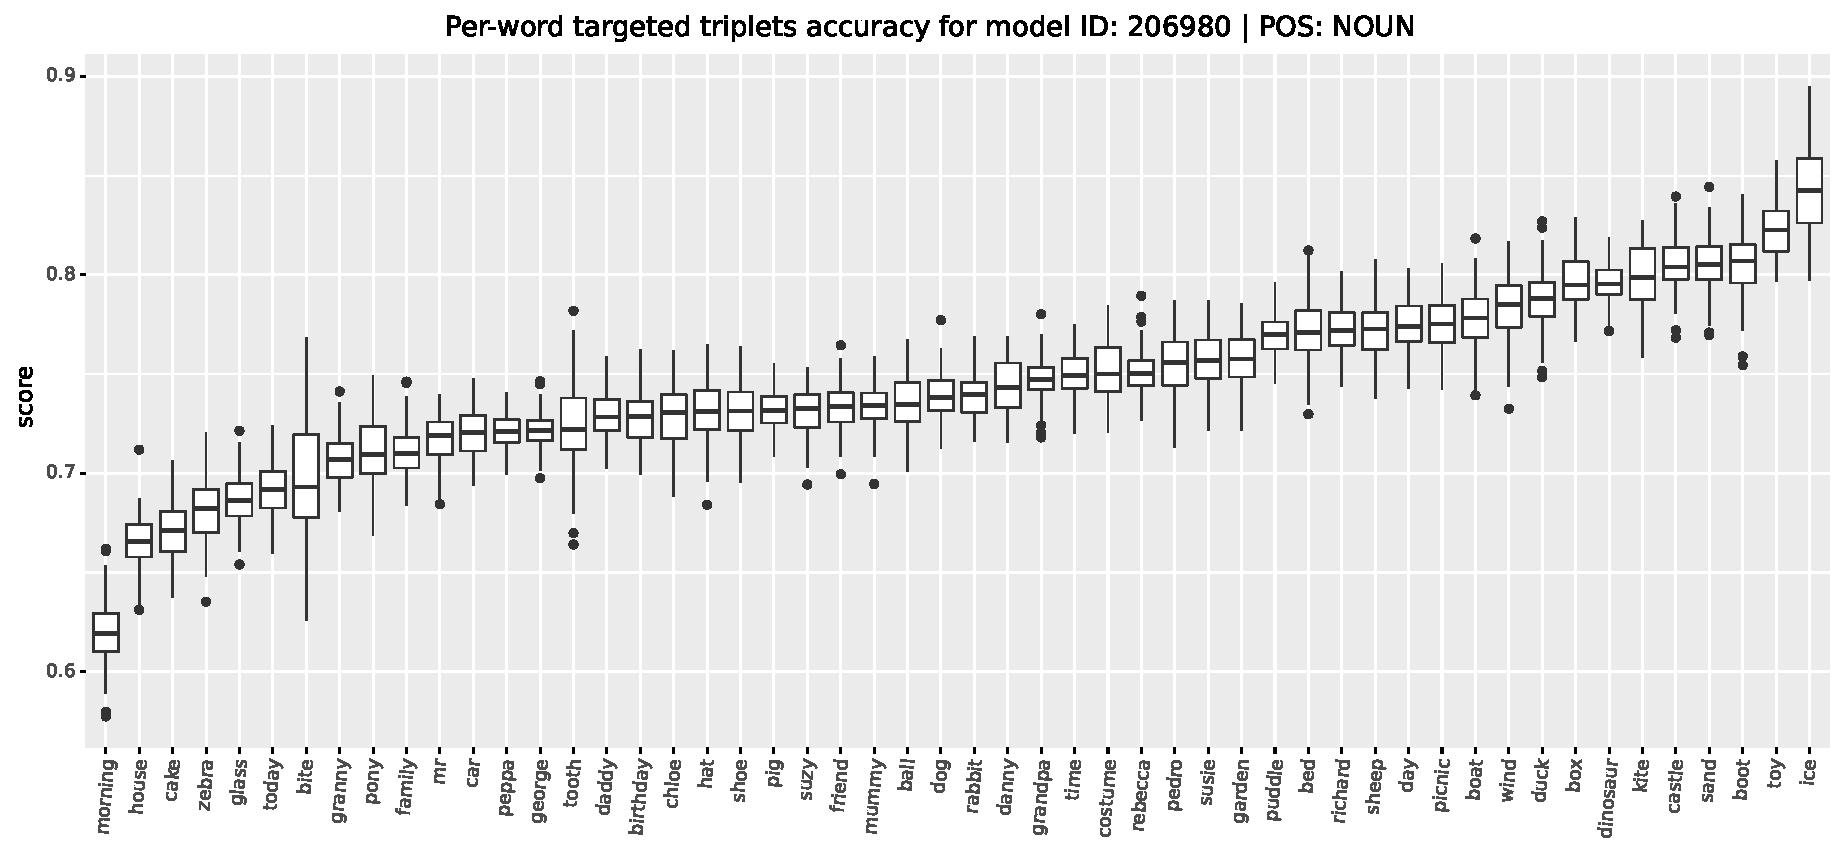
\includegraphics[width=\textwidth]{results/targeted_triplets/results_per_word_version_206980_NOUN.pdf}
  \caption{Per-word targeted triplets accuracy for nouns.}
  \label{fig:accuracy_targeted_triplets_nouns}
\end{figure*}

\begin{figure*}[htb]
  \centering
  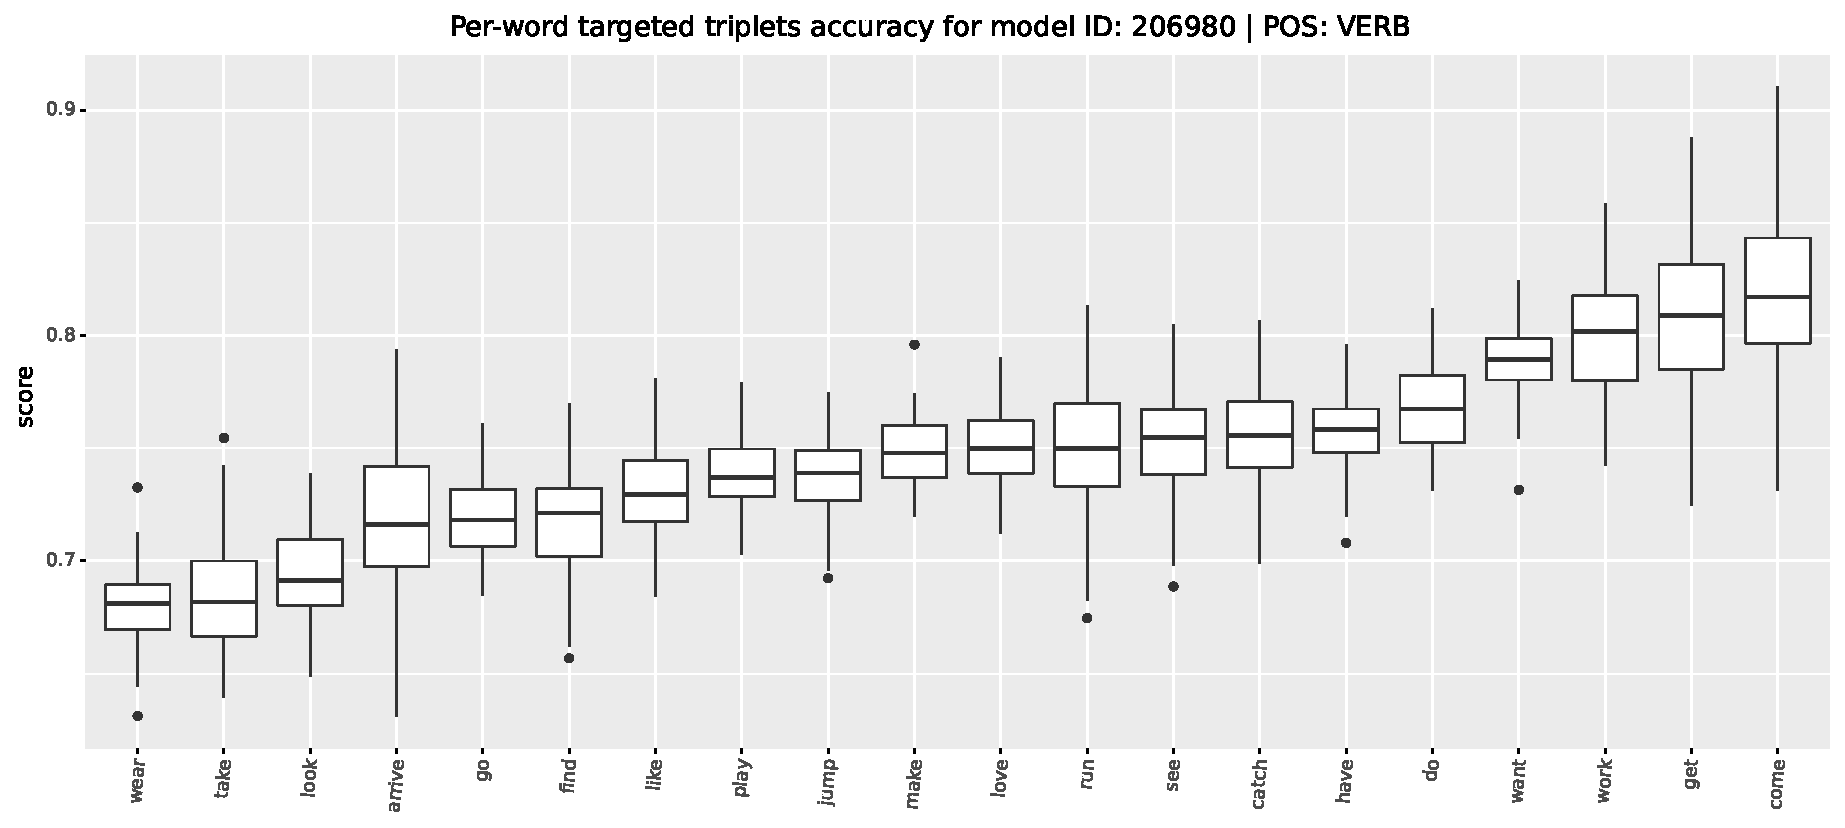
\includegraphics[width=\textwidth]{results/targeted_triplets/results_per_word_version_206980_VERB.pdf}
  \caption{Per-word targeted triplets accuracy for verbs.}
  \label{fig:accuracy_targeted_triplets_verbs}
\end{figure*}
